\documentclass[mathserif]{beamer}

\usepackage{parskip}
\usepackage{amsmath}
\usepackage{amssymb}
\usepackage{graphicx}

\frenchspacing

\logo{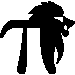
\includegraphics[width=0.075\textwidth]{../Logo}}

\usetheme{Rochester}
\usecolortheme{whale}
%\beamertemplatenavigationsymbolsempty

\AtBeginSection[] {%
	\begin{frame}
		\frametitle{Table of Contents}
		\tableofcontents[currentsection]
	\end{frame}
}

\newenvironment{compactmath}[1][\normalsize]%
	{\begin{minipage}{\textwidth}\vspace{-0.75\baselineskip}#1\begin{equation*}}
	{\end{equation*}\end{minipage}}

\newenvironment{namedframe}[1]%
	{\begin{frame}\frametitle{#1}\framesubtitle{\secname}}
	{\end{frame}}


\title{Introduction to Sets}
\author{Vincent Macri}
\date{
\includegraphics{../LicenseLogo}\\\copyright{} Vincent Macri, 2017}

\newcommand{\such}{\ |\ }

\begin{document}
	\frame{\titlepage}
	\section{Types of Numbers}
	\begin{namedframe}{Basic types}
		\begin{description}
			\item[$\mathbb{N}$] Natural numbers ($0, 1, 2, 3, \dots$)
			\item[$\mathbb{Z}$] Integers ($\mathbb{N} \text{ and } {-1}, -2, -3, \dots$)
			\item[$\mathbb{Q}$] Rational numbers ($\mathbb{Z} \text{ and } 4.2, -\frac{2}{3}, \dots$)
			\item[$\mathbb{R}$] Real numbers ($\mathbb{Q} \text{ and } \pi, e, \sqrt{2}, \dots$)
			\item[$\mathbb{C}$] Complex numbers ($\mathbb{R} \text{ and } i, 2i + 1, \dots$)
			\item[$\mathbb{P}$] Prime numbers ($2, 3, 5, 7, \dots$)
		\end{description}
	\end{namedframe}
	\begin{namedframe}{Indexes}
		Some mathematicians include 0 in $\mathbb{N}$, and some do not.

		While it is generally accepted that $\mathbb{N}$ includes 0, we have notation to specify:
		\begin{description}
			\item[$\mathbb{N}^0$] Natural numbers including 0
			\item[$\mathbb{N}^*$] Natural numbers not including 0
			\item[$\mathbb{N}^+$] Positive natural numbers (does not include 0)
		\end{description}

		We can also use this notation with other types of numbers:
		\begin{description}
			\item[$\mathbb{Z}^-$] Negative integers (does not include 0)
			\item[$\mathbb{R}^+$] Positive real numbers (does not include 0)
		\end{description}
	\end{namedframe}
	\section{Intervals}
	\begin{namedframe}{Open and closed}
		\begin{block}{Open intervals}
			To denote numbers in an open (inclusive) range, we write: $[a, b]$

			This means all the real numbers from $a$ to $b$, including $a$ and $b$.
		\end{block}
		\begin{block}{Closed intervals}
			To denote numbers in a closed (exclusive) range, we write: $(a, b)$

			This means all the real numbers from $a$ to $b$, \alert{not} including $a$ and $b$.
		\end{block}
	\end{namedframe}
	\begin{namedframe}{Examples}
		\begin{description}
			\item [$[0, 10)$] means all real numbers from 0 to 10, including 0, but not including 10.
			\item [$(-\infty, +\infty)$] means all real numbers.
			\item [$[0, \infty)$] means all real numbers that are not negative.
		\end{description}
	\end{namedframe}
	\section{Sets}
	\begin{namedframe}{Basics}
		A set is an unordered collection of distinct elements.

		A set with a finite number of elements can be written in braces such as $\{a, b, c, \dots\}$

		For example, we can define the set of math club co-presidents as:
		\[M = \{\text{Vincent}, \text{Samantha}, \text{Caroline}\}\]
		By convention, the names of sets are denoted in capital letters.

		Since the elements of a set are distinct:
		\[\{a, b, c\} \equiv \{a, a, b, c, b\}\]
		($\equiv$ means equivalent)
	\end{namedframe}
	\begin{namedframe}{The empty set}
		The empty set is the set that contains no elements. It is denoted as $\varnothing$.
		
		\begin{examples}
			$\varnothing$ is the set of all 4-sided triangles.

			$\varnothing$ is the set of all prime numbers divisible by 10.
		\end{examples}
		The empty set can be thought of as an empty bag. It may be empty, but it still exists.
		\begin{block}{Definition}
			\begin{compactmath}[\Huge]
				\varnothing = \{\}
			\end{compactmath}
		\end{block}
	\end{namedframe}
	\begin{namedframe}{Subsets and supersets}
		A set $A$ is a subset of a set $B$ if all elements of $A$ are in $B$.

		A set $B$ is a superset of a set $A$ if all elements of $A$ are in $B$.

		\sep

		We write that $A$ is a subset of $B$ as: $A \subseteq B$.

		We write that $B$ is a superset of $A$ as: $B \supseteq A$.

		\sep

		What if $A \subseteq B$ and $B \subseteq A$?

		\pause

		Then $A = B$.

		\sep

		\begin{block}{Quick trick}
			A set with $k$ elements has $2^k$ different subsets.
		\end{block}
	\end{namedframe}
	\begin{namedframe}{Cardinality}
		The cardinality of a set is the size of a set.

		\sep

		For example, the cardinality of the set $A = \{u, 1, c\}$ is \pause$3$.

		We write this as $n(A) = 3$.
	\end{namedframe}
	\section{Notation}
	\begin{namedframe}{Set membership}
		Recall our set of co-presidents:
		\[M = \{\text{Vincent}, \text{Samantha}, \text{Caroline}\}\]
		
		To say that an element is in a set, we use the symbol $\in$, meaning ``is an element of'', ``belongs to'', or (informally) ``in''.
		\[\therefore \text{Vincent} \in M\]
		To say that an element is not in a set, we use the symbol $\notin$, meaning ``is not an element of'', ``does not belong to'', or (informally) ``not in''.
		\[\therefore \text{Euler} \notin M\]
	\end{namedframe}
	\begin{namedframe}{Set-builder notation}
		For more complex sets, we can define them using set-builder notation.

		For example, we can define the set of even numbers as so:
		\[E = \{x\ |\ (\exists k \in \mathbb{Z})[x = 2k]\}\]
		\textbar{} reads as ``such that''

		$\exists$ reads as ``there exists''

		This reads as: ``$E$ is the set of $x$ values such that there exists an integer $k$ such that $x = 2k$'' (the second ``such that'' is implied).

		\scriptsize
		Sometimes, set-builder notation can get complicated. Using words to define a set is also valid, but you must be careful that you are \alert{not} ambiguous with your wording!
	\end{namedframe}
	\begin{namedframe}{The universe of discourse}
		The universe of discourse (commonly shortened to universe) is the set of all values under consideration. It is similar to the domain of a function.

		The universe set is commonly denoted as $U$.
		\begin{example}[Defining $\mathbb{P}$]
			\begin{compactmath}
				U = \{x\ |\ x \in \mathbb{N}^*, x \neq 1\}
			\end{compactmath}
			\[\mathbb{P} = \{x\ |\ x \in U \text{ and the only positive divisors of $x$ are $1$ and $x$}\}\]
			If we had instead defined $U$ as $U = \mathbb{Z}$, then our definition of primes would include negative numbers, which would be wrong. This is why it is important to consider the universe of discourse.
		\end{example}
	\end{namedframe}
	\section{Operations with Sets}
	\begin{namedframe}{Set union}
		The union of two sets is a set containing all of the elements of both sets.
		\\
		The set union operator is: $\cup$

		Formally:
		\[A \cup B = \{x\ |\ x \in A \vee x \in B\} \qquad \text{($\vee$ means ``or'')}\]

		For example:
		\[A = \{1, 2, 3\}\]
		\[B = \{3, 4, 5\}\]
		\[A \cup B = \{1, 2, 3, 4, 5\}\]
	\end{namedframe}
	\begin{namedframe}{Set intersection}
		The intersection of two sets is a set containing only the elements that are in both sets.
		\\
		The set intersection operator is: $\cap$

		Formally:
		\[A \cap B = \{x\ |\ x \in A \wedge x \in B\} \qquad \text{($\wedge$ means ``and'')}\]

		For example:
		\[A = \{1, 2, 3\}\]
		\[B = \{3, 4, 5\}\]
		\[A \cap B = \{3\}\]
	\end{namedframe}
	\begin{namedframe}{Set complement}
		The \alert{complement} of the set $A$ is all elements not in $A$.

		If the universe, $U$, is defined, the \alert{absolute complement} of $A$ is all elements in $U$ that are not in $A$.
		
		The \alert{relative complement} of $A$ with respect to $B$ is written as $B \setminus A$. This is the set of elements in $B$, but not in $A$.
		\begin{block}{Definition}
			\begin{compactmath}[\large]
				B \setminus A = \{x \in B\ |\ x \notin A\}
			\end{compactmath}
		\end{block}
		\pause
		\begin{examples}
			\begin{compactmath}
				\{1, 2, 3, 4, 5\} \setminus \{4, 5, 6, 7, 8\} = \{1, 2, 3\}
			\end{compactmath}
			\begin{compactmath}
				\mathbb{R} \setminus \mathbb{Q} = \{x\ |\ x \text{ is irrational}\}
			\end{compactmath}
		\end{examples}
	\end{namedframe}
	\begin{namedframe}{Cartesian product}
		The Cartesian product of a set $A$ with a set $B$ is defined as:
		\[A \times B = \{(a,b) \such a \in A \wedge b \in B\}\]

		\sep

		For example, if $A = \{1,2,3\}$ and $B = \{a,b,c\}$, what is $A \times B$?

		\pause

		\[A \times B = \{(1,a),(1,b),(1,c),(2,a),(2,b),(2,c),(3,a),(3,b),(3,c)\}\]
	\end{namedframe}
\end{document}
